\documentclass[11pt,a4paper]{article}
\usepackage[T1]{fontenc}
\usepackage[utf8]{inputenc}
\usepackage[english]{babel}
\usepackage[margin=2.2cm]{geometry}
\usepackage{booktabs,tabularx,array}
\usepackage{tikz}
\usetikzlibrary{arrows.meta,positioning}
\usepackage[hidelinks]{hyperref}
\usepackage{enumitem}
\setlist[itemize]{nosep,leftmargin=*}
\setlength{\parindent}{0pt}
\setlength{\parskip}{5pt}
\renewcommand{\arraystretch}{1.15}
\newcolumntype{Y}{>{\raggedright\arraybackslash}X}
\tikzset{box/.style={draw,rounded corners,align=center,text width=3.6cm,minimum height=0.75cm,font=\small},link/.style={-{Stealth},thick}}

\begin{document}
\begin{center}
{\LARGE\bfseries WEEKLY PROGRESS REPORT}\par
{\large Vietnamese Text Classification: UIT-VSMEC}\par
Reporting period: 7--14 October 2026\par
Student: \underline{\hspace{5cm}}\quad Group: NLP
\end{center}

\section{Weekly objective}
The instructor assigned further work on UIT-VSMEC, including TF-IDF, word embeddings, SVM, BiLSTM, and ViSoBERT. The instruction places model training after the study stage and further guidance from the instructor.

My project work focused on preparing the data pipeline and the BiLSTM implementation. I also prepared validation, test evaluation, and an integration test. The report uses repository commits from 8--11 October and the current working files. Some changes are uncommitted, so their exact completion dates are not established by the commit history.

\section{Work completed in the project}
\subsection{Data loading and UIT-VSMEC support}
I separated data loading from the main program. The 11 October commit records this change. The current loader supports both the existing UIT-VSFC task and UIT-VSMEC through a dataset option.

For UIT-VSMEC, the loader converts the source fields \texttt{Sentence} and \texttt{Emotion} into the fields used by the existing pipeline. It maps seven emotion labels to numeric targets: Anger, Disgust, Enjoyment, Fear, Other, Sadness, and Surprise. These are the labels configured in the project code.

I prepared separate training, validation, and test loaders with a batch size of 32. The vocabulary is built only from training sentences. Validation and test sentences therefore cannot add words to the training vocabulary. UIT-VSMEC has no topic target in this implementation, so the batch uses a placeholder that the training function ignores.

\subsection{Text preparation and word embeddings}
I prepared lowercasing and Vietnamese word tokenization with \texttt{underthesea}. The preprocessing code builds a vocabulary, converts tokens to numeric IDs, and pads sequences within each batch. It reserves IDs for padding and unknown words. Empty token sequences receive an unknown token to keep the model input valid.

The BiLSTM uses a trainable embedding layer with 512 dimensions. This provides a working implementation of the word-embedding route in the assignment. The current model does not load pretrained word vectors.

\subsection{BiLSTM model preparation}
I prepared a three-layer bidirectional LSTM with 512 hidden units per direction. The model handles variable-length inputs through packed sequences. It combines the final forward and backward hidden states before applying a linear classification layer.

The output size depends on the selected dataset. This allows the same model class to support three UIT-VSFC labels or seven UIT-VSMEC labels.

\subsection{Training and evaluation code}
I prepared a training loop with cross-entropy loss and Adam at a learning rate of \texttt{0.001}. The script is configured for five epochs and selects CUDA when available. It keeps the weights with the highest validation accuracy and evaluates those weights on the test split.

I added accuracy and macro-averaged precision, recall, and F1 calculations. The 8 October commit also records the addition of a test function. These are implementation outputs; they do not establish that a full training run was completed.

\section{Progress against the assigned criteria}
\begin{tabularx}{\textwidth}{@{}p{2.6cm}p{2.6cm}Y@{}}
\toprule
\textbf{Criterion} & \textbf{Current status} & \textbf{Project evidence or remaining work}\\
\midrule
UIT-VSMEC & Implemented in code & Dataset selection, field conversion, label mapping, and three split loaders.\\
TF-IDF & Remaining topic & No TF-IDF implementation or study notes were found in the inspected project files.\\
Word embeddings & Implemented in code & Trainable embedding layer, vocabulary, token IDs, padding, and sequence lengths.\\
SVM & Remaining topic & No SVM implementation or study notes were found in the inspected project files.\\
BiLSTM & Implemented in code & Bidirectional sequence model with dataset-dependent output size.\\
ViSoBERT & Remaining topic & No ViSoBERT implementation or study notes were found in the inspected project files.\\
Training results & Not recorded & Training code exists, but no saved run metrics were found in the inspected files.\\
\bottomrule
\end{tabularx}

The remaining-topic status describes the available project evidence. It does not rule out reading or other work completed outside the repository.

\section{Implementation structure}
The diagram shows the current processing order. Training and evaluation are available in code; their presence does not confirm a completed experiment.
\begin{center}
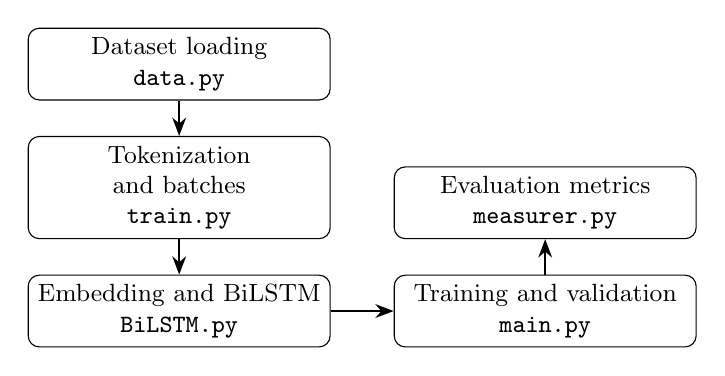
\begin{tikzpicture}[node distance=0.45cm and 0.8cm]
\node[box] (data) {Dataset loading\\\texttt{data.py}};
\node[box,below=of data] (tokens) {Tokenization and batches\\\texttt{train.py}};
\node[box,below=of tokens] (model) {Embedding and BiLSTM\\\texttt{BiLSTM.py}};
\node[box,right=of model] (run) {Training and validation\\\texttt{main.py}};
\node[box,above=of run] (metrics) {Evaluation metrics\\\texttt{measurer.py}};
\draw[link] (data)--(tokens);
\draw[link] (tokens)--(model);
\draw[link] (model)--(run);
\draw[link] (run)--(metrics);
\end{tikzpicture}
\end{center}

\section{Relationship to the research assignment}
The graph maps the assigned representations to the model routes under consideration. Dashed arrows indicate routes that remain to be studied or implemented. It contains no measured performance values.
\begin{center}
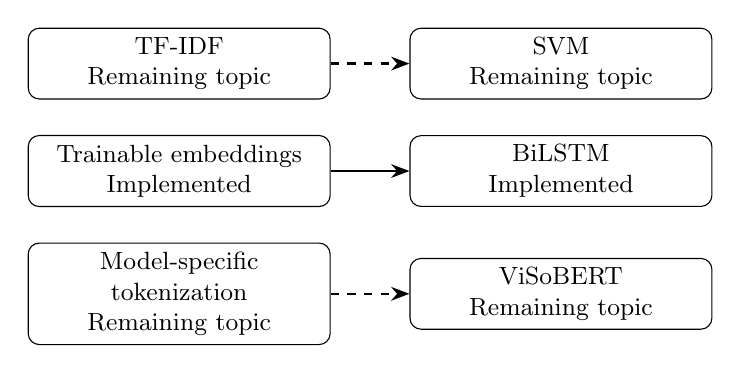
\begin{tikzpicture}[node distance=0.45cm and 1cm]
\node[box] (tfidf) {TF-IDF\\Remaining topic};
\node[box,right=of tfidf] (svm) {SVM\\Remaining topic};
\node[box,below=of tfidf] (emb) {Trainable embeddings\\Implemented};
\node[box,right=of emb] (lstm) {BiLSTM\\Implemented};
\node[box,below=of emb] (tok) {Model-specific tokenization\\Remaining topic};
\node[box,right=of tok] (bert) {ViSoBERT\\Remaining topic};
\draw[link,dashed] (tfidf)--(svm);
\draw[link] (emb)--(lstm);
\draw[link,dashed] (tok)--(bert);
\end{tikzpicture}
\end{center}

\section{Verification and limits}
The existing integration test was run during report preparation with:
\begin{quote}
\texttt{python -m unittest test\_data.py}
\end{quote}
One test passed, covering both dataset options through local test data. It checks target IDs, unknown-word handling, missing topic handling, model output size, a finite loss, and backpropagation. This check confirms those integration paths. It does not download and verify the complete datasets or measure classification quality.

No accuracy, precision, recall, or F1 results are reported because no saved experiment results were found. The instructor's message requires further guidance before training. The existing training script is therefore reported as preparation work.

\section{Next week's plan}
\begin{enumerate}[nosep,leftmargin=*]
\item Complete the study notes for TF-IDF and SVM, including how they can form a baseline for the selected dataset.
\item Study ViSoBERT input preparation and the steps needed to adapt it to the classification task.
\item Confirm the dataset version, label mapping, evaluation criteria, and experiment settings with the instructor.
\item After further instruction, run the agreed experiments and save the settings and evaluation results for comparison.
\end{enumerate}
\end{document}
